\chapter{Calculations of $\pi_1(X)$}
In this chapter, we will calculate the fundamental group of various topological spaces.

More explicitly, we begin with a simplicial complex $K$ and its topological realization $X = |K|$. For $b \in X$, we will study \({\pi }_{1}\left( {X,b}\right)\) by the combinatorial structure of $K$.

\begin{definition} [Edge Loop] Let \(K = \left( {V,\Sigma }\right)\) be a simplicial complex.

\begin{enumerate}
    \item An edge path \(\left( {{v}_{0},\ldots,{v}_{n}}\right)\) is such that

(a) \({a}_{i} \in  V\left( K\right)\)

(b) For each \(i,\left\{  {{a}_{i - 1},{a}_{i}}\right\}\) spans a simplex of \(K\)

\item An edge loop is an edge path with \({a}_{n} = {a}_{0}\).

\item Let \(\alpha  = \left( {{v}_{0},\ldots,{v}_{n}}\right),\beta  = \left( {{w}_{0},\ldots,{w}_{m}}\right)\) be two edge paths with \({v}_{n} = {w}_{0}\), then we define
\[
\alpha  \circ  \beta  = \left( {{v}_{0},\ldots,{v}_{n},{w}_{1},\ldots,{w}_{m}}\right)
\]
\end{enumerate}
\end{definition}

\begin{definition} [Elementary Contraction/Expansion] Let \(\alpha,\beta\) be two edge paths.

 \begin{enumerate}
     \item An elementary contraction of \(\alpha\) is a new edge path obtained by performing one of the following on \(\alpha\):

\begin{itemize}
\item Replacing \(\cdots {a}_{i - 1}{a}_{i}\cdots\) by \(\cdots {a}_{i - 1}\cdots\) provided that \({a}_{i - 1} = {a}_{i}\)

\item Replacing \(\cdots {a}_{i - 1}{a}_{i}{a}_{i + 1}\cdots\) by \(\cdots {a}_{i - 1}\cdots\) provided that \({a}_{i - 1} = {a}_{i + 1}\)

\item Replacing \(\cdots {a}_{i - 1}{a}_{i}{a}_{i + 1}\cdots\) by \(\cdots {a}_{i - 1}{a}_{i + 1}\cdots\) provided that \(\left\{  {{a}_{i - 1},{a}_{i},{a}_{i + 1}}\right\}\) spans a 2-simplex of \(K\).
\end{itemize}

\item An elementary expansion is the reverse of the elementary contraction.

\item Two edge paths \(\alpha,\beta\) are equivalent if \(\alpha\) and \(\beta\) differs by a finite sequence of elementary contractions or expansions.

\item The equivalence class of edge loops is given by:
\[
\left\lbrack  \alpha \right\rbrack   = \left\{  {{\alpha }^{\prime } \mid  {\alpha }^{\prime } \sim  \alpha,{\alpha }^{\prime }\text{ is the edge loop based at }b}\right\}
\]
\end{enumerate}
\end{definition}

Note that \({\alpha }^{\prime } \sim  \alpha\) if they differ from finitely many elementary contractions or expansions. For instance, let \(K\) in the figure below denote a triangle:
\begin{center}
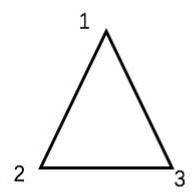
\includegraphics[width=0.25\textwidth]{images/Ch8_triangle123.jpg}
\end{center}
Then the canonical form of any equivalence form \(\left\lbrack  \alpha \right\rbrack\) can be expressed as:
\[
\left\lbrack  \alpha \right\rbrack   = \left\lbrack  {{bcabc}\cdots {ab}}\right\rbrack ,
\]
where \(a,b,c \in  \{ 1,2,3\}\) are distinct.

\begin{proposition} Let 
\begin{center}
\(E\left( {K,b}\right):= \{ \left\lbrack  \alpha \right\rbrack   \mid  \alpha\) is edge loop based at \(b\}\) 
\end{center}
Then $E\left( {K,b}\right)$ is a group with multiplication
\[
\left\lbrack  \alpha \right\rbrack   * \left\lbrack  \beta \right\rbrack   = \left\lbrack  {\alpha  \cdot  \beta }\right\rbrack
\]
We call $E(K,b)$ the \emph{edge loop group based at} $b$.
\end{proposition}

\begin{proof}
1. Well-definedness: Note that by definition,
\[
\alpha  \sim  {\alpha }^{\prime },\beta  \sim  {\beta }^{\prime } \Rightarrow  \alpha  \cdot  \beta  \sim  {\alpha }^{\prime } \cdot  {\beta }^{\prime }
\]
2. Associativity is clear.

\noindent 3. The identity is \(e = \left\lbrack  b\right\rbrack\): for any edge loop \(\left\lbrack  \alpha \right\rbrack   = \left\lbrack  {b{v}_{1}\cdots b}\right\rbrack\),

\[
\left\lbrack  \alpha \right\rbrack   * e = \left\lbrack  {b{v}_{1}\cdots {v}_{n}b}\right\rbrack   * \left\lbrack  b\right\rbrack
= \left\lbrack  {b{v}_{1}\cdots {v}_{n}{bb}}\right\rbrack
= \left\lbrack  {b{v}_{1}\cdots {v}_{n}b}\right\rbrack   = \left\lbrack  \alpha \right\rbrack .\]
Also, \(e * \left\lbrack  \alpha \right\rbrack   = \left\lbrack  \alpha \right\rbrack\).

\noindent 4. The inverse of any edge loop \(\left\lbrack  {b{v}_{1}\cdots {v}_{n}b}\right\rbrack\) is \(\left\lbrack  {b{v}_{n}\cdots {v}_{1}b}\right\rbrack\):
\begin{align*}
{\left\lbrack  b{v}_{1}\cdots {v}_{n}b\right\rbrack  }^{-1} * \left\lbrack  {b{v}_{1}\cdots {v}_{n}b}\right\rbrack  &= \left\lbrack  {b{v}_{n}\cdots {v}_{1}{bb}{v}_{1}\cdots {v}_{n}b}\right\rbrack
\\
&= \left\lbrack  {b{v}_{n}\cdots {v}_{1}b{v}_{1}\cdots {v}_{n}b}\right\rbrack
\\
&= \left\lbrack  {b{v}_{n}\cdots {v}_{2}{v}_{1}{v}_{2}\cdots {v}_{n}b}\right\rbrack
\\
&= \cdots
\\
&= \left\lbrack  b\right\rbrack
\end{align*}
Similarly, \(\left\lbrack  {b{v}_{1}\cdots {v}_{n}b}\right\rbrack   * {\left\lbrack  b{v}_{1}\cdots {v}_{n}b\right\rbrack  }^{-1} = \left\lbrack  b\right\rbrack\).
\end{proof}

Indeed, the edge loop group of a simplicial complex gives us a combinatorial way of studying the fundamental group of its topological realization: 
\begin{theorem} \label{thm:edge_loop_fundamental}
\(E\left( {K,b}\right)  \cong  {\pi }_{1}\left( {\left| K\right|,b}\right)\).
\end{theorem} 

This is the most difficult theorem that we have faced so far. To do so, we recall (a slight generalization of) the simplicial approximation theorem (\autoref{thm:simplicial_approx}): Suppose that \(f\): \(\left| K\right|  \rightarrow  \left| L\right|\) be such that for all \(v \in  V\left( K\right)\), there exists \(g\left( v\right)  \in  V\left( L\right)\) satisfying
\[
f\left( {{\operatorname{st}}_{K}\left( v\right) }\right)  \subseteq  {\operatorname{st}}_{L}\left( {g\left( v\right) }\right).
\]
Then there is a simplicial map
\(g: \;K \rightarrow  L
\)
with $v \mapsto  g\left( v\right)$
and \(\left| g\right|  \simeq  f\).

A generalization of the simplicial approximation theorem needed for the proof of \autoref{thm:edge_loop_fundamental} is as follows: if \(A \subseteq  K\)
and \(B \subseteq  L\) are simplicial subcomplexes, and \[f\left( \left| A\right| \right)  \subseteq  \left| B\right|,\] 
then the above \(g\) can be chosen such that 
\[{\left. g\right| }_{A}: A \rightarrow  B\] 
and the homotopy \(\left| g\right|  \simeq  f\) sends \(\left| A\right|\) to \(\left| B\right|\).

\begin{proof} For each edge loop \(\alpha  = \left( {{v}_{0},\ldots,{v}_{n}}\right)\) based at \(b\), consider the simplicial complex
\begin{center}
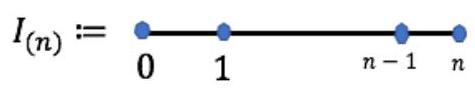
\includegraphics[width=0.4\textwidth]{images/Ch8_n_segments.jpg}
\end{center}
together with the simplicial map
\[
{g}_{\alpha }: \;{I}_{\left( n\right) } \rightarrow  K
\quad \text{ with }{g}_{\alpha }\left( i\right)  = {v}_{i}.
\]
Note that it is well-defined, since \(\{ i,i + 1\}  \in  \Sigma_{{I}_{\left( n\right) }}\), and \(\left\{  {{v}_{i},{v}_{i + 1}}\right\}   \in  \Sigma_{K}\).

Now construct the mapping
\begin{center}
\(\theta : \;\{ \alpha\ |\ \alpha \) edge loop based at \(b\}  \rightarrow  {\pi }_{1}\left( {K,b}\right)\)
\end{center}
by 
\[\alpha  \mapsto  \left\lbrack  \left| {g}_{\alpha }\right| \right\rbrack,\]
where \(\left| {g}_{\alpha }\right| : \left| {I}_{\left( n\right) }\right| \left( { \cong  \left\lbrack  {0,1}\right\rbrack  }\right)  \rightarrow  \left| K\right|\)
satisfies
\(\left| {g}_{\alpha }\right| \left( {i/n}\right)  = {v}_{i}\).

For example, let $K$ be given by
\begin{center}
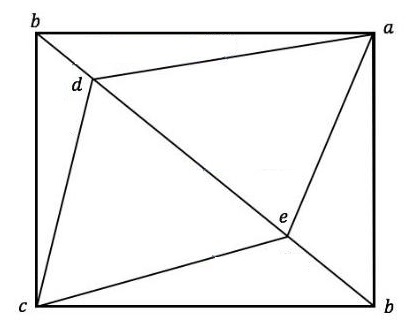
\includegraphics[width=0.4\textwidth]{images/Ch8_edge_loop.jpg}
\end{center}
and $\alpha  = \left( \text{ bdeabcb }\right)$, then the simplicial map $g_{\alpha}: I_{(6)} \to K$
has realization given by:
\[
\left| {g}_{\alpha }\right| \left( 0\right)  = b,\left| {g}_{\alpha }\right| \left( {1/6}\right)  = d,\left| {g}_{\alpha }\right| \left( {2/6}\right)  = e,\cdots,\left| {g}_{\alpha }\right| \left( 1\right)  = b,
\]
So \(\left| {g}_{\alpha }\right|\) is a loop based at \(b\), and \(\left\lbrack  \left| {g}_{\alpha }\right| \right\rbrack   \in  {\pi }_{1}\left( {\left| K\right|,b}\right)\).

Now, suppose \(\alpha  \sim  {\alpha }^{\prime }\) be two edge loops differ by an elementary contraction, e.g.,
\[
{\alpha }^{\prime } = \left( \text{ bdebcb }\right)  \sim  \alpha  = \left( \text{ bdeabcb }\right).
\]
Then one can easily find a homotopy \(\left| {g}_{{\alpha }^{\prime }}\right|  \simeq  \left| {g}_{\alpha }\right|\) relative to \(\{ 0,1\}\). As a result, \(\left\lbrack  \left| {g}_{\alpha }\right| \right\rbrack   = \left\lbrack  \left| {g}_{{\alpha }^{\prime }}\right| \right\rbrack\), and we have a well-defined map:
\begin{center}
\(\widetilde{\theta }: \;\{\) edge loops based at \(b\}  / \sim\   := E\left( {K,b}\right)\rightarrow  {\pi }_{1}\left( {\left| K\right|,b}\right)\)
\end{center}
with \(\left\lbrack  \alpha \right\rbrack   \mapsto  \left\lbrack  \left| {g}_{\alpha }\right| \right\rbrack\).

Now we show \(\widetilde{\theta }\) {\bf is a homomorphism}, i.e.
\[
\widetilde{\theta }\left( {\left\lbrack  \alpha \right\rbrack   * \left\lbrack  \beta \right\rbrack  }\right)  = \widetilde{\theta }\left( \left\lbrack  \alpha \right\rbrack  \right) \widetilde{\theta }\left( \left\lbrack  \beta \right\rbrack  \right),
\]
which suffices to show \(\left\lbrack  \left| {g}_{\alpha  \cdot  \beta }\right| \right\rbrack   = \left\lbrack  {\left| {g}_{\alpha }\right| \left| {g}_{\beta }\right| }\right\rbrack\), i.e., \(\left| {g}_{\alpha  \cdot  \beta }\right|  \simeq  \left| {g}_{\alpha }\right| \left| {g}_{\beta }\right|\). Note that \(\left| {g}_{\alpha  \cdot  \beta }\right|\) and \(\left| {g}_{\alpha }\right| \left| {g}_{\beta }\right|\) are the same path with different "speeds", therefore, one can easily construct a homotopy between the maps.

Next, we show \(\widetilde{\theta }\) {\bf is surjective}: Let \(\ell : \left\lbrack  {0,1}\right\rbrack   \rightarrow  \left| K\right|\) be a loop based at \(b\). It suffices to find an edge loop \(\alpha\) such that \(\left\lbrack  \left| {g}_{\alpha }\right| \right\rbrack   = \left\lbrack  \ell \right\rbrack\), i.e., \(\left| {g}_{\alpha }\right|  \simeq  \ell\).

To do so, apply the simplicial approximation theorem such that there exist a large \(n\) and \(g: {I}_{\left( n\right) } \rightarrow  K\) such that \(\left| g\right|  \simeq  \ell\). Here we can choose \(g: {I}_{\left( n\right) } \rightarrow  K\) to be such that \(g\left( 0 \right)  = b =  g\left( n \right)\), and \(\left| g\right|  \simeq  \ell\) relative to \(\{ 0,1\}\). Then one can take 
\[\alpha  = \left( {g\left( 0\right),g\left( 1\right),\ldots,g\left( n\right) }\right),\] 
so that \(g\left( 0\right)  = b = g\left( n\right)\), with \({g}_{\alpha } = g\). Therefore, \(\left\lbrack  \left| {g}_{\alpha }\right| \right\rbrack   = \left\lbrack  \ell \right\rbrack\), and hence \(\widetilde{\theta }\) is surjective.

Now we show that $\overline{\theta}$ {\bf is injective}: Let \(\alpha  = \left( {{v}_{0},\ldots,{v}_{n}}\right)\) be an edge loop based at \(b\) such that \(\theta \left( \left\lbrack  \alpha \right\rbrack  \right)  = e\), i.e., \(\left| {g}_{\alpha }\right|  \simeq  {c}_{b}\). It suffices to show that \(\left\lbrack  \alpha \right\rbrack\) is the identity element of \(E\left( {K,b}\right)\).

Choose a homotopy \(H: I \times  I \rightarrow  \left| K\right|\) 
between \(\left| {g}_{\alpha }\right|  \simeq  {c}_{b}\):
\begin{center}
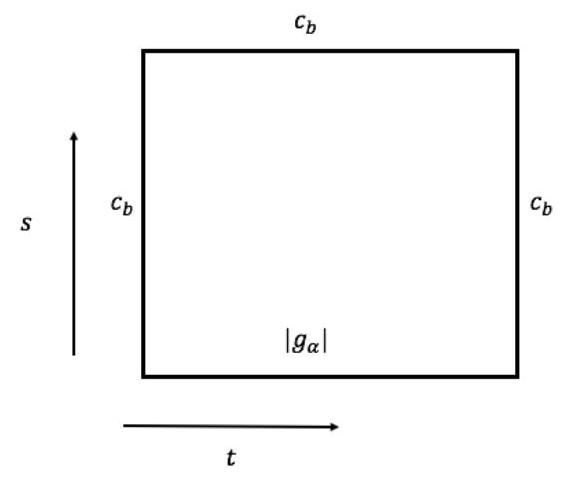
\includegraphics[width=0.4\textwidth]{images/Ch8_g_alpha_cb.jpg}
\end{center}
\hspace*{3em} 
Apply the simplicial approximation theorem on $H$, so that there exists a subdivision \({\left( I \times  I\right) }_{\left( r\right) }\) of \(I \times  I\) with $r \times r$ squares:
\begin{center}
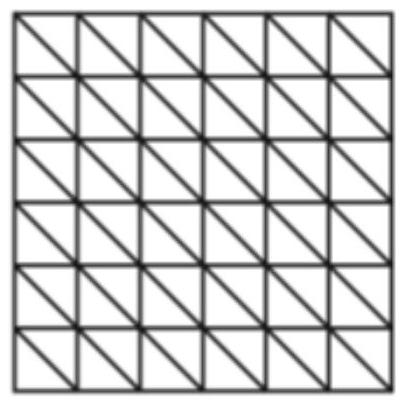
\includegraphics[width=0.35\textwidth]{images/Ch8_Irr.jpg}
\end{center}
such that \(\left| {\left( I \times  I\right) }_{\left( r\right) }\right|  \cong I \times  I\) are isomorphic, and there exists a simplicial map
\[
G:{\left( I \times  I\right) }_{\left( r\right) } \rightarrow  K
\ \text{  such that }\ \left| G\right|  \simeq  H\text{. }
\]
Without loss of generality, assume that \(r\) is a sufficiently large multiple of \(n\). Then the graphic illustration of \(\left| G\right|\) is:
\begin{center}
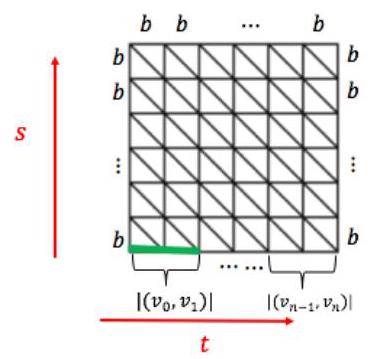
\includegraphics[width=0.4\textwidth]{images/Ch8_bar_G.jpg}
\end{center}
\vspace{-3mm}
In particular, \(\left| G\right|\) maps \(\{ 0,1\}  \times  I\) into \(\{ b\} ;I \times  \{ 1\}\) into \(\{ b\} ;\left( {i/n,0}\right)\) into \(\left\{  {v}_{i}\right\} ,i = 0,\ldots,n\), and \(\left\lbrack  {i/n,\left( {i + 1}\right) /n}\right\rbrack\) into \(\left| \left( {{v}_{i},{v}_{i + 1}}\right) \right|,i = 0,\ldots,n - 1\).

Now look at the green line (with $\eta:=r/n$ vertices) at the bottom of $|G|$: it is the path from $v_0 = b$ to $v_1$, i.e.
$$G(0,0) = v_0 = b, \quad \dots, \quad G(0,\gamma/r) = v_1$$
and hence $G$ defines an edge path
\[
\left(G(0,0),\ G(0,\frac{1}{n}), \dots, G(0,\frac{\gamma-1}{n}),\ G(0,\frac{\gamma}{n})\right) = (b = v_0, v_0, \dots, v_0, v_1, \dots, v_1).
\]
As a result, the edge loop corresponding to the bottom edge of the square reads 
\[\left(G(0,0), G(0,\frac{1}{n}), \dots, G(0,\frac{n-1}{n}), G(0,1)\right) = \left( {b{v}_{0}\cdots {v}_{0}{v}_{1}\cdots {v}_{1}\cdots {v}_{n}\cdots {v}_{n}b}\right)\]
and clearly
\[
\beta  \sim  \left( {b{v}_{0}{v}_{1}{v}_{2}\cdots {v}_{n - 1}{v}_{n}b}\right)
\sim  \left( {b{v}_{1}{v}_{2}\cdots {v}_{n - 1}b}\right)  = \alpha, 
\]
i.e. $[\beta] = [\alpha] \in E(K,b)$. So it suffices to show \(\beta  \sim  e\) as edge loops, which can be seen by the sequence of elementary contractions and expansions:
\vspace{-2mm}
\begin{center}
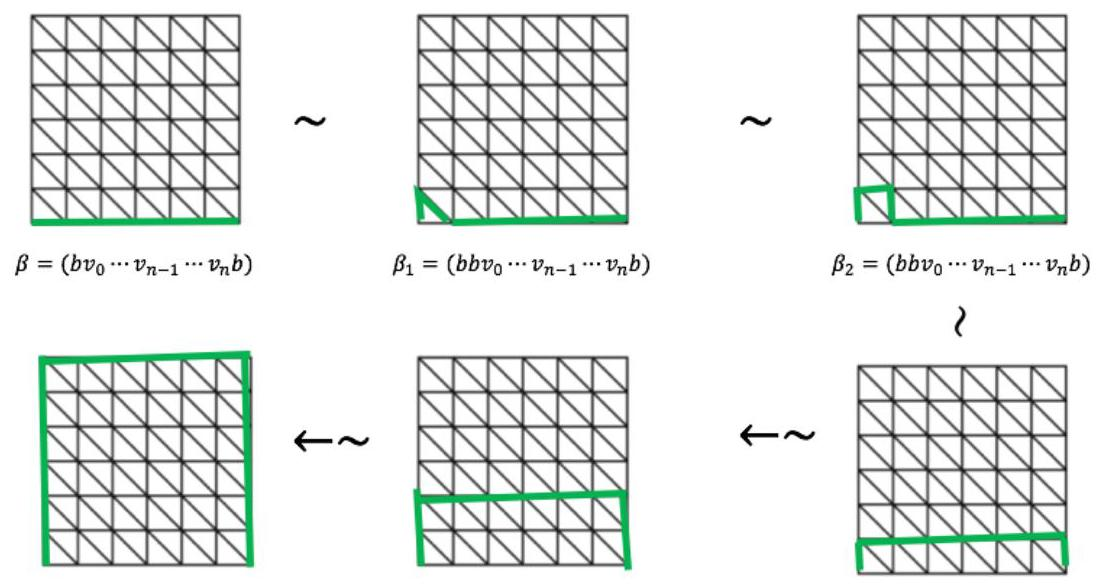
\includegraphics[width=0.7\textwidth]{images/Ch8_edge_equivalence.jpg}
\end{center}
By tracing the above elementary contractions, one has \(\beta  \sim  \left( {b\cdots b}\right)  = \left( b\right)\) on the bottom left hand picture, and hence $[\beta] = e$.
\end{proof}

Note that the definition of \(E\left( {K,b}\right)\) only involves \(n\) -simplicials for \(n \leq  2\), so one has:
\begin{proposition} For any simplicial complex \(K\), consider the simplicial subcomplex \({\operatorname{Skel}}^{n}\left( K\right)  = \left( {{V}_{k},\Sigma_{K}^{n}}\right)\), where \(\Sigma_{K}^{n}\) consists of \(\sigma  \in  \Sigma_{K}\) with \(\left| \sigma \right|  \leq  n + 1\) (this is the \(n\)-skeleton of \(K\) ). Then
\[
{\pi }_{1}\left( {\left| K\right|,b}\right)  \cong  {\pi }_{1}\left( {\left| {{\operatorname{Skel}}^{2}\left( K\right) }\right|,b}\right)
\]
\end{proposition}
\begin{proof} Since \(E\left( {K,b}\right)\) only involves \(n\) -simplicials for \(n \leq  2\), we imply \(E\left( {K,b}\right)  \cong  E\left( {{\operatorname{Skel}}^{2}\left( K\right),b}\right)\).

Moreover, \({\pi }_{1}\left( {\left| K\right|,b}\right)  \cong  E\left( {K,b}\right)\) and \({\pi }_{1}\left( {\left| {{\operatorname{Skel}}^{2}\left( K\right) }\right|,b}\right)  \cong  E\left( {{\operatorname{Skel}}^{2}\left( K\right),b}\right)\). So the proof is complete.
\end{proof}

\begin{corollary} \label{cor:Sn_simply_connected} For \(n \geq  2,{\pi}_{1}\left({S}^{n}\right)\) is simply connected.
\end{corollary}

\begin{proof} Consider the simplicial complex \(K\) with
\[
V = \{ 1,2,\ldots,n + 2\},\;\Sigma  = \{ \text{ all proper subsets of }V\}
\]
It is clear that \(\left| K\right|  \cong \Delta^n \cong  {S}^{n}\), and \({\operatorname{Skel}}^{2}\left( K\right)\) has

\begin{itemize}
\item \(V: \{ 1,\ldots,n + 2\}\)
\item \(\Sigma^{2}\): all subsets of \(V\) with less or equal to 3 elements.
\end{itemize}
For any edge loop \(a\) in \({\pi }_{1}\left( \left| {{\operatorname{skel}}^{2}\left( K\right) }\right| \right)\), we have
\[
a = \left( {b{v}_{0}{v}_{1}{v}_{2}\cdots {v}_{n}}\right)
\sim  \left( {b{v}_{1}{v}_{2}\cdots {v}_{n - 2}{v}_{n - 1}b}\right)
\sim \dots \sim  \left( b\right)
\]
Therefore, all edge loops \(\alpha\) in \({\pi }_{1}\left( \left| {{\operatorname{skel}}^{2}\left( K\right) }\right| \right)\) satisfies \(\left\lbrack  \alpha \right\rbrack   = \left\lbrack  \left( b\right) \right\rbrack   = e\)., i.e.,
\[
{\pi }_{1}\left( \left| {{\operatorname{skel}}^{2}\left( K\right) }\right| \right)  \cong  \{ e\}
\]
which implies \({\pi }_{1}\left( \left| K\right| \right)  \cong  {\pi }_{1}\left( \left| {{\operatorname{skel}}^{2}\left( K\right) }\right| \right)  \cong  \{ e\}\). Since \(\left| K\right|  \cong  {S}^{n}\), we have
\[
{\pi }_{1}\left( {S}^{n}\right)  \cong  {\pi }_{1}\left( \left| K\right| \right)  \cong  \{ e\}.
\]
\end{proof}

\section{Fundamental Group of $S^1$}
\autoref{cor:Sn_simply_connected} does not hold for \({S}^{1}\), since the constructed \(\Sigma^{2}\) for \({S}^{1}\) does not contain \(\{ 1,2,3\}\). Instead, we have
\begin{theorem} \({\pi }_{1}\left( {S}^{1}\right)  \cong  \mathbb{Z}\).
\end{theorem}
\begin{proof} Consider the simplicial complex \(K\) below with $|K| \cong S^1$:
\begin{center}
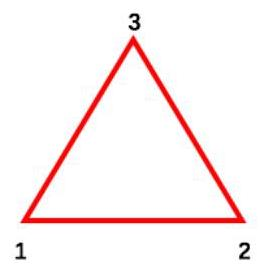
\includegraphics[width=0.25\textwidth]{images/Ch8_triangle.jpg}
\end{center}
It suffices to show \(E\left( {K,1}\right)  \cong  \mathbb{Z}\). Define the orientation of \(\left| K\right|\) as shown below.
\begin{center}
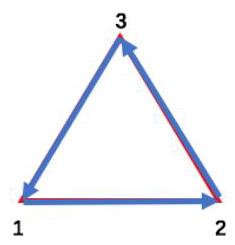
\includegraphics[width=0.25\textwidth]{images/Ch8_triangle_oriented.jpg}
\end{center}
We construct the isomorphism between \(E\left( {K,b}\right)\) and \(\mathbb{Z}\) directly:
\begin{center}
\(\phi : \;E\left( {K,b}\right)  \rightarrow  \mathbb{Z}\)
with \(\left\lbrack  \alpha \right\rbrack   \mapsto\) winding number of \(\alpha\)
\end{center}
where the winding number of \(\alpha\) is 
\begin{center}
number of times it traverses $(2,3)$ $-$ number of times it traverses $(3,2)$.
\end{center}
Note that:

1. The winding number for \(\left( {1{23}\cdots {123}1}\right)  = m\), where $23$ shows up for \(m\) times

2. The winding number for \(\left( {1{32}\cdots {132}1}\right)  =  - n\), where $32$ shows up for \(n\) times

3. The winding number is invariant under elementary contractions and elementary expansions, since (for instance) $(1231321) \sim (123321) \sim (1221) \sim (1)$, that is, the $32$ and $23$ `cancel out' each other.

Therefore, any edge loop \(\alpha\) based at $1$ is equivalent uniquely to one of the canonical form:
\[
\alpha  \sim  \left( {{1bc1bc}\cdots {1bc1}}\right),\;\text{ where }{bc} = {32}\text{ or 23. }
\]
and $\phi: E(K,1) \to \mathbb{Z}$ is well-defined.

To see $\phi$ is a homomorphism, consider any two edge loops \(\alpha,\beta\) based at $1$. suppose that \(\left\lbrack  \alpha \right\rbrack   = \left\lbrack  \left( {{1bc1bc}\cdots {1bc1}}\right) \right\rbrack\) and \(\left\lbrack  \beta \right\rbrack   = \left\lbrack  \left( {{1pq1pq}\cdots {1pq1}}\right) \right\rbrack\) are at their canonical forms, then
\[
\phi \left( {\left\lbrack  \alpha \right\rbrack   \cdot  \left\lbrack  \beta \right\rbrack  }\right)  = \phi \left( \left\lbrack  {\alpha  \cdot  \beta }\right\rbrack  \right)  = \left\lbrack  \left( {{1bc1bc}\cdots {1bc11pq1pq}\cdots {1pq1}}\right) \right\rbrack
\]
Then one can easily check that
$\phi \left( {\left\lbrack  \alpha \right\rbrack   \cdot  \left\lbrack  \beta \right\rbrack  }\right) = \phi \left( {\left\lbrack  \alpha \right\rbrack  }\right) + \phi \left(  \left\lbrack  \beta \right\rbrack  \right)$.
Moreover, it is easy to see that $\phi$ is bijective. 
Therefore, \(\phi\) is an isomorphism.
\end{proof}

Actually, we can show that the loop based at 1 given by:
\[
\ell \;I \rightarrow  {S}^{1}
\text{ with }t \mapsto  {e}^{2\pi it}
\]
is a generator for \({\pi }_{1}\left( {{S}^{1},1}\right)\).



\begin{corollary} [Fundamental Theorem of Algebra] All non-constant polynomials in \(\mathbb{C}\) has at least one root in \(\mathbb{C}\).
\end{corollary}
\begin{proof} Suppose on the contrary that
\[
p\left( x\right)  = {a}_{n}{x}^{n} + \cdots  + {a}_{1}x + {a}_{0} \neq  0
\]
has no complex roots, then \(p\) is a continuous mapping from \(\mathbb{C}\) to \(\mathbb{C} \smallsetminus  \{ 0\}\). 

It is clear that \(\mathbb{C} \smallsetminus  \{ 0\}  \simeq  \{ z \in \mathbb{C} \mid  \left| z\right|  = 1\}\), and therefore
\(
{\pi }_{1}\left( {\mathbb{C}\smallsetminus \{ 0\} }\right)  = {\pi }_{1}\left( {S}^{1}\right)  \cong  \mathbb{Z}.
\), and the induced homomorphism \({p}_*\) of \(p\) is given by:
\[
{p}_{ * }: \;{\pi }_{1}\left( \mathbb{C}\right) \cong \{e\} \rightarrow  {\pi }_{1}\left( {\mathbb{C}\smallsetminus \{ 0\} }\right) \cong \mathbb{Z}
\]
Since $p_*$ is a group homomorphism, \({p}_{ * }\left( e\right)  = 0\).

Consider the inclusion 
$i: \;{C}_{r} \hookrightarrow  \mathbb{C}$, where \({C}_{r} = \{ z \in  \mathbb{C}\left| \right| z \mid   = r\}\) is the circle of radius $r$, and consider
the diagram given below: Or equivalently,
\begin{center}
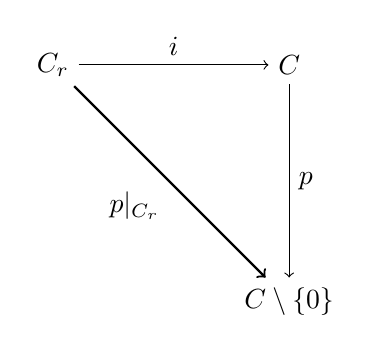
\begin{tikzpicture}[node distance=3cm, auto]
  \node (A) {$C_r$};
  \node (B) [right of=A] {$\mathbb{C}$};
  \node (C) [below of=B] {$\mathbb{C} \setminus \{0\}$};
  \draw[->] (A) to node {$i$} (B);
  \draw[->,thick] (A) to node [swap] {$p|_{C_r}$} (C);
  \draw[->] (B) to node {$p$} (C);
\end{tikzpicture}
\end{center}
As a result, the induced homomorphism \({i}_{ * }\) of \(i\) satisfies the diagram

\begin{center}
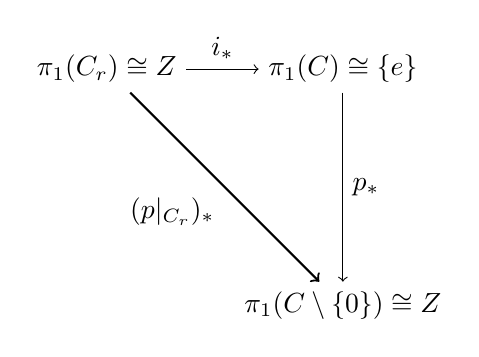
\begin{tikzpicture}[node distance=3cm, auto]
  \node (A) {$\pi_1(C_r) \cong \mathbb{Z}$};
  \node (B) [right of=A] {$\pi_1(\mathbb{C}) \cong \{e\}$};
  \node (C) [below of=B] {$\pi_1(\mathbb{C} \setminus \{0\}) \cong \mathbb{Z}$};
  \draw[->] (A) to node {$i_*$} (B);
  \draw[->,thick] (A) to node [swap] {$(p|_{C_r})_*$} (C);
  \draw[->] (B) to node {$p_*$} (C);
\end{tikzpicture}
\end{center}
Therefore, \({p}_{ * } \circ  {i}_{ * }\) is a zero map since \({p}_{ * }\left( e\right)  = 0\), i.e., \({\left( {\left. p\right| }_{{C}_{r}}\right) }_{ * }\) is a zero homomorphism.

Now study \({\left. p\right| }_{{C}_{r}}: {C}_{r} \rightarrow  \mathbb{C} \smallsetminus  \{ 0\}\). Construct
\[ q\left( z\right)  = k \cdot  {z}^{n},\ \text{ where } k \mathrel{\text{:= }} \frac{p\left( r\right) }{{r}^{n}}
\]
Then \({\left. p\right| }_{{C}_{r}},{\left. q\right| }_{{C}_{r}}: {C}_{r} \rightarrow  \mathbb{C} \smallsetminus  \{ 0\}\) with \(p\left( r\right)  = q\left( r\right)\).

We {\bf claim} that \({\left. p\right| }_{{C}_{r}} \simeq  {\left. q\right| }_{{C}_{r}}\) for large \(r\): First construct the mapping
\[
H: \;{C}_{r} \times  \left\lbrack  {0,1}\right\rbrack   \rightarrow  \mathbb{C}
\ \text{ with }H\left( {z,t}\right)  = {tp}\left( z\right)  + \left( {1 - t}\right) q\left( z\right)
\]
and $H\left( {z,0}\right)  = q\left( z\right),H\left( {z,1}\right)  = p\left( z\right)$. 
If 
\[H: {C}_{r} \times  \left\lbrack  {0,1}\right\rbrack   \rightarrow  \mathbb{C} \smallsetminus  \{ 0\}\]
i.e. $H(z,t) \neq 0$ for all $z \in C_r$ and $t \in [0,1]$, \(H\) defines a homotopy between \({\left. p\right| }_{{C}_{r}}\) and \({\left. q\right| }_{{C}_{r}}\).

Suppose on the contrary that there exists $(z, t)$ such that
\[
\left( {1 - t}\right) p\left( z\right)  + {tq}\left( z\right)  = 0,\;\left| z\right|  = r,t \in  \left\lbrack  {0,1}\right\rbrack
\]
Or equivalently,
\[
\left( {1 - t}\right) \left( {{a}_{n}{z}^{n} + \cdots  + {a}_{1}z + {a}_{0}}\right)  + t \cdot  k{z}^{n} = 0.
\]
Substituting \(k\) with \(p\left( r\right) /{r}^{n}\) gives

\[
{a}_{n}{z}^{n} + \cdots  + {a}_{1}z + {a}_{0} = t\left( {{a}_{n - 1}{z}^{n - 1} + \cdots  + {a}_{0} - {a}_{n - 1}\frac{{z}^{n}}{r} - \cdots  - {a}_{1}\frac{{z}^{n}}{{r}^{n - 1}} - {a}_{0}\frac{{z}^{n}}{{r}^{n}}}\right)
\]

The LHS has leading order \(n\), while the RHS has leading order less or equal to \(n - 1\). As \(r = \left| z\right|  \rightarrow  \infty,t \rightarrow  \infty\). Therefore, the equality does not hold in the range \(t \in  \left\lbrack  {0,1}\right\rbrack\) when \(r\) is sufficiently large, and the claim is proved for $r$ sufficiently large.

Therefore, \({\left. p\right| }_{{C}_{r}} \simeq  {\left. q\right| }_{{C}_{r}}\) and \({\left( {\left. p\right| }_{{C}_{r}}\right) }_{ * } = {\left( {\left. q\right| }_{{C}_{r}}\right) }_{ * }\). 

Consider the induced mapping \({\left( {\left. q\right| }_{{C}_{r}}\right) }_{ * }: \mathbb{Z} \rightarrow  \mathbb{Z}\). In particular, we check the value of \({\left( {\left. q\right| }_{{C}_{r}}\right) }_{ * }\left( 1\right)\), where 1 is the generator in \({\pi }_{1}\left( {C}_{r}\right)\).

Recall that the loop
\(\ell : \;I \rightarrow  {C}_{r}
\)
with \(\ell \left( t\right)  = r{e}^{2\pi it}
\) is a generator of $\pi_1(C_r) \cong \mathbb{Z}$, i.e. \(\left\lbrack  \ell \right\rbrack   = 1\). It follows that
\[
{\left( {\left. q\right| }_{{C}_{r}}\right) }_{ * }\left( 1\right)  = {\left( {\left. q\right| }_{{C}_{r}}\right) }_{ * }\left( \left\lbrack  \ell \right\rbrack  \right)  = \left\lbrack  {{\left. q\right| }_{{C}_{r}}\left( \ell \right) }\right\rbrack   = q\left( {r{e}^{2\pi it}}\right)  = k \cdot  {r}^{n} \cdot  {e}^{2\pi int} \neq  0.
\]

Therefore, \({\left( {\left. q\right| }_{{C}_{r}}\right) }_{ * }: \mathbb{Z} \cong  {\pi }_{1}\left( {C}_{r}\right)  \rightarrow  {\pi }_{1}\left( {\mathbb{C}\backslash \{ 0\} }\right)  \cong\)  \(\mathbb{Z}\) is the nonzero map \(1 \mapsto  n\), contradicting the fact that \({\left( {\left. q\right| }_{{C}_{r}}\right) }_{ * } = {\left( {\left. p\right| }_{{C}_{r}}\right) }_{ * }\) is the zero homomorphism.
\end{proof}

\section{Fundamental Group of a Graph}

\begin{definition} [Graph] A graph \(T = \left( {V,E}\right)\) is defined by the following components:

\begin{itemize}
\item \(V\) is a finite or countable set, called vertex set;

\item \(E\) is a finite or countable set, called edge set;
\item A function \(\delta : E \rightarrow  V \times  V\) with \(\delta \left( e\right)  = \left( {\ell \left( e\right),\tau \left( e\right) }\right)\), where \(\ell \left( e\right),\tau \left( e\right)\) is known as the endpoints of \(e\).
\end{itemize}
\end{definition}

\begin{example} 1. Let \(V = \{ 1\},E = \left\{  {{e}_{1},{e}_{2},{e}_{3}}\right\}\), and define \(\delta \left( {e}_{i}\right)  = \left( {1,1}\right),i = 1,2,3\). The graph $(V, E)$ is represented below:
\begin{center}
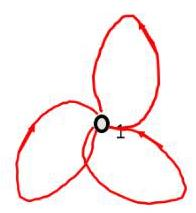
\includegraphics[width=0.3\textwidth]{images/Ch8_3_petal.jpg}
\end{center}

2. Let \(V = \left\{  1,2,3\right\}\) and \(E = \left\{  {{e}_{1},\ldots,{e}_{6}}\right\}\), and define
\[
\delta \left( {e}_{1}\right)  = \left( {1,1}\right),\;\delta \left( {e}_{2}\right)  = \left( {1,2}\right),\;\delta \left( {e}_{3}\right)  = \left( {1,2}\right),
\delta \left( {e}_{4}\right)  = \left( {2,3}\right),\;\delta \left( {e}_{5}\right)  = \left( {2,3}\right),\;\delta \left( {e}_{6}\right)  = \left( {3,3}\right).
\]
The graph $(V, E)$ is represented below (We do not care the direction of edges for this graph):
\begin{center}
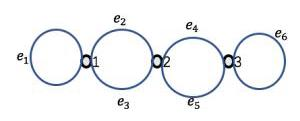
\includegraphics[width=0.5\textwidth]{images/Ch8_4_circles.jpg}
\end{center}
\end{example}

\begin{definition} [Realization of a Graph] For a given graph \(\Gamma  = \left( {V,E}\right)\), construct a realization by
\[
\{ \left| V\right|  \times  \{ \text{ zero simplices }\} \coprod \left| E\right|  \times  \{ 1\text{ -simplices } \} / \sim
\]
where the equivalence class is induced from the function \(\delta\). We still call this realization of the graph as \(\Gamma\).
\end{definition}

In general, graphs are not simplicial complexes. But we can "sub-divide" each edge of \(\Gamma\) into three parts such that there exists simplicial complex \(K\) with \(\left| K\right|  \cong  \Gamma\). For instance,
\begin{center}
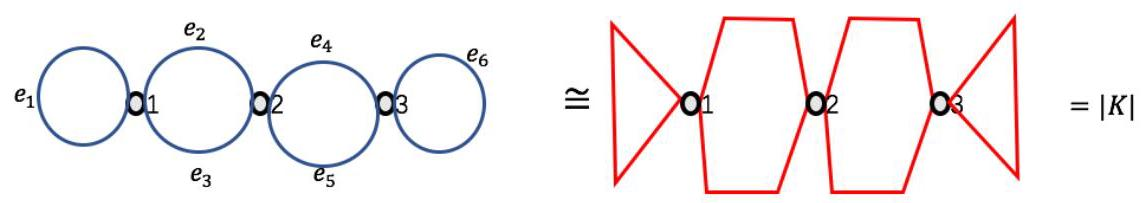
\includegraphics[width=0.9\textwidth]{images/Ch8_simp_cplx.jpg}
\end{center}

\begin{definition}
Let $\Gamma = (V,E)$ be a graph:
\begin{itemize}
\item A \emph{subgraph} \({\Gamma }^{\prime } \subseteq  \Gamma\) is \({\Gamma }^{\prime } = \left( {{V}^{\prime },{E}^{\prime }}\right)\) with \({V}^{\prime } \subseteq  V\) and \({E}^{\prime } \subseteq  E\), and
\[
\delta { \mid  }_{{V}^{\prime }}: {E}^{\prime } \rightarrow  {V}^{\prime } \times  {V}^{\prime }
\]
\item An \emph{edge path} is a continuous function \(p: \left\lbrack  {0,1}\right\rbrack   \rightarrow  \Gamma\) such that there exists \(n \in  \mathbb{N}\) satisfying
\[
{\left. p\right| }_{\left\lbrack  i/n,i + 1/n\right\rbrack  }: \left\lbrack  {\frac{i}{n},\frac{i + 1}{n}}\right\rbrack   \rightarrow  T
\]
is a path along an edge of \(\Gamma\), or a constant function on a vertex of \(\Gamma\), for \(0 \leq  i \leq  n - 1\).
\end{itemize}
\end{definition}

Under the homeomorphism \(\Gamma  \cong  \left| K\right|\), each edge path is homotopic to \(\left| {g}_{\alpha }\right|\) for some edge path \(\alpha\) in the simplicial complex \(K\). For instance:
\begin{center}
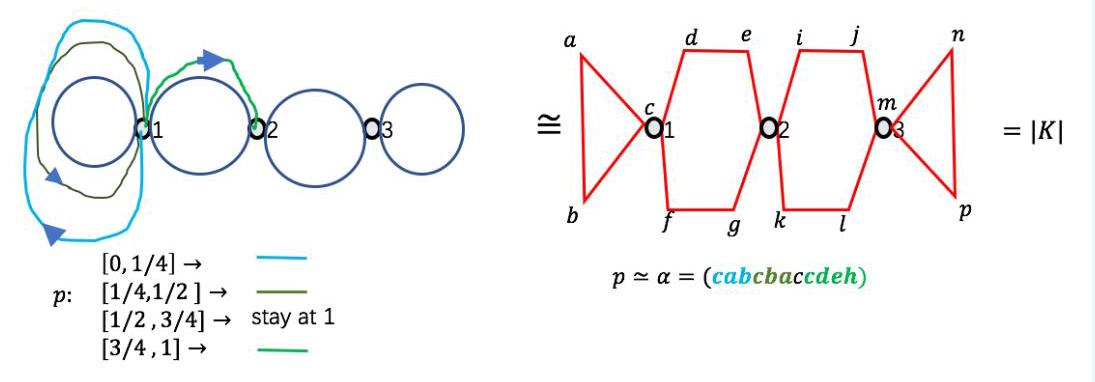
\includegraphics[width=1\textwidth]{images/Ch8_edge_path_approx.jpg}
\end{center}

Here are more definitions:
\begin{definition}
Let $\Gamma = (V,E)$ be a graph:
\begin{itemize}
\item An edge loop is an edge path \(p\) such that \(p\left( 0\right)  = p\left( 1\right)  = b \in  V\).
\item An embedded edge loop is an injective edge loop, i.e., \(p: \left\lbrack  {0,1}\right\rbrack   \rightarrow  \Gamma\) such that for \(x \notin  V,\;{p}^{-1}\left( x\right)  = \varnothing\) or a single point.
\item A tree is a connected graph \(T\) that contains no embedded edge loop \(p: \left\lbrack  {0,1}\right\rbrack   \rightarrow  T\). For instance, as shown in the figure, \({T}_{1}\) contains no edge loop, in particular, the edge loop $(a, b, a)$ is not embedded; \({T}_{2}\) contains embedded edge loop $(a, b, c, d, a)$.

\item Maximal Tree of a connected graph \(\Gamma\) is a subgraph \(T\) of \(\Gamma\) such that 
\begin{itemize}
    \item \(T\) is a tree; and 
    \item By adding an edge \(e \in  E\left( \Gamma \right)  \smallsetminus  E\left( T\right)\) into \(T\), the new graph is no longer a tree.
\end{itemize}
 \end{itemize}
 \end{definition}


For instance, \(T \subseteq  \Gamma\) shown in the figure below is a maximal tree.
\begin{center}
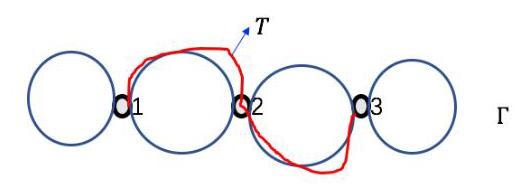
\includegraphics[width=0.4\textwidth]{images/Ch8_maximal_tree.jpg}
\end{center}

With all the definitions given above, we can finally compute the fundamental group of a (connected) graph:
\begin{theorem} \label{thm:max_tree_exists} Let \(\Gamma\) be a connected graph, and \(T\) is a subgraph of \(\Gamma\) such that \(T\) is a tree. Then \(T\) is a maximal tree if and only if \(V\left( T\right)  = V\left( \Gamma \right)\).

Moreover, there always exists a maximal tree for all \(\Gamma\).
\end{theorem}

\begin{proof} Outline for second part: Construct an ordering of \(\left\{  {{v}_{1},\ldots,{v}_{i}}\right\}   \subseteq  V\left( \Gamma \right)\), such that for each integer \(i \geq  2\), there is an edge connecting \({v}_{i + 1}\) with some vertex in \(\left\{  {{v}_{1},\ldots,{v}_{i}}\right\}\).
Then construct 
\[{T}_{1} \subseteq  {T}_{2} \subseteq  \cdots,\] 
where \({T}_{i}\) is a tree containing vertices \(\left\{  {{v}_{1},\ldots,{v}_{i}}\right\}\). As a result, \(T = { \cup  }_{i \in  \mathbb{N}}{T}_{i}\) is a maximal tree.
\end{proof}


\begin{theorem} Let \(\Gamma\) be a connected graph. Then \(\pi \left( \Gamma \right)\) is isomorphic to the free group generated by \(\# \{ E\left( \Gamma \right)  \smallsetminus  E\left( T\right) \}\) elements, for any maximal tree of \(\Gamma\).
\end{theorem}


For instance, a maximal tree of the the graph \(T \subseteq  {\Gamma }_{1}\) is: 
\begin{center}
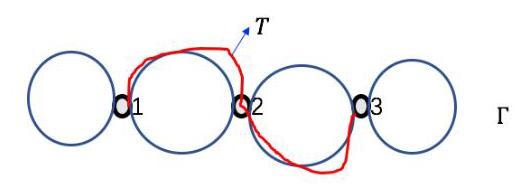
\includegraphics[width=0.5\textwidth]{images/Ch8_maximal_tree.jpg}
\end{center}
Therefore, \({\pi }_{1}\left( {\Gamma }_{1}\right)  \cong  \langle a,b,c,d\rangle\) since \(\# \left\{  {E\left( {\Gamma }_{1}\right)  \smallsetminus  E\left( T\right) }\right\}   = 4\).

On the other hand, a maximal tree of the graph with `4-petals' \(T \subseteq  {\Gamma }_{2}\) is just the middle vertexc:
\begin{center}
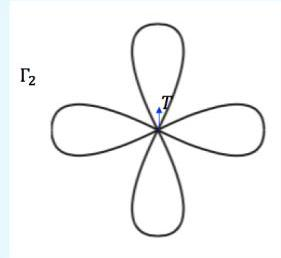
\includegraphics[width=0.3\textwidth]{images/Ch8_4_petals.jpg}
\end{center}
Therefore, \({\pi }_{1}\left( {\Gamma }_{2}\right)  \cong  \langle a,b,c,d\rangle\) since \(\# \left\{  {E\left( {\Gamma }_{2}\right)  \smallsetminus  E\left( T\right) }\right\}   = 4\).

Indeed, one has \({\Gamma }_{1} \simeq  {\Gamma }_{2}\). The reason for such homotopy equivalence is in the link

https://www.math3ma.com/blog/clever-homotopy-equivalences

\bigskip
We will not prove the theorem. Instead, we present the idea of the proof in the special case of \(\Gamma\) with the following specified maximal tree $T$ and orientation:
\begin{center}
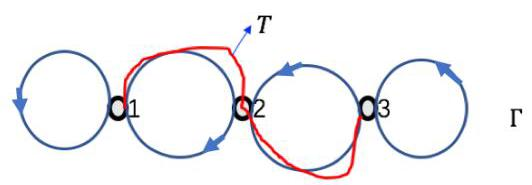
\includegraphics[width=0.6\textwidth]{images/Ch8_maximal_tree_oriented.jpg}
\end{center}
and the simplicial complex $K$ with \(\left| K\right|  \cong  \Gamma\):
\begin{center}
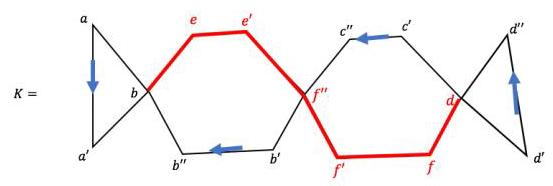
\includegraphics[width=0.6\textwidth]{images/Ch8_simp_approx_oriented.jpg}
\end{center}
Now we construct the group homomorphism
\[
\phi : \;\langle \alpha,\beta,\gamma,\delta \rangle  \rightarrow  E\left( {K,b}\right)  \cong  {\pi }_{1}\left( \Gamma \right)
\]
with 
\begin{align*} \phi \left( \alpha \right)  &= \left\lbrack  {b{a}^{\prime }{a}^{\prime \prime }b}\right\rbrack\\ 
\phi \left( \beta \right)  &= \left\lbrack  {{be}{e}^{\prime }{f}^{\prime \prime }{b}^{\prime }{b}^{\prime \prime }b}\right\rbrack \\
\phi \left( \gamma \right)  &= \left\lbrack  {{be}{e}^{\prime }{f}^{\prime \prime }{f}^{\prime }{fd}{c}^{\prime }{c}^{\prime \prime }{f}^{\prime \prime }{e}^{\prime }{eb}}\right\rbrack
\\
\phi \left( \delta \right)  &= \left\lbrack  {{\text{ bee }}^{\prime }{f}^{\prime \prime }{f}^{\prime }{fd}{d}^{\prime \prime }{d}^{\prime }{df}{f}^{\prime }{f}^{\prime \prime }{e}^{\prime }{eb}}\right\rbrack
\end{align*}
We can show the group homomorphism \(\phi\) is bijective. In particular, the inverse of \(\phi\) is given by:
\[
\Psi : \;E\left( {K,b}\right)  \rightarrow  \langle \alpha,\beta,\gamma,\delta \rangle
\]
where for any \(\left\lbrack  \ell \right\rbrack   \mathrel{\text{:= }} \left\lbrack  {b{v}_{1}\cdots {v}_{n}}\right\rbrack   \in  E\left( {K,b}\right)\), the mapping \(\Psi \left\lbrack  \ell \right\rbrack\) is constructed by

(a) Remove all other letters appearing in \(\ell\) except \(b,{a}^{\prime },{a}^{\prime \prime },{b}^{\prime },{b}^{\prime \prime },{c}^{\prime },{c}^{\prime \prime },{d}^{\prime },{d}^{\prime \prime }\)

(b) Assign
\[
\alpha,{\alpha }^{-1},\beta,{\beta }^{-1},\gamma,{\gamma }^{-1},\delta,{\delta }^{-1}
\]
for each appearance of
\[
{a}^{\prime }{a}^{\prime \prime },{a}^{\prime \prime }{a}^{\prime },{b}^{\prime }{b}^{\prime \prime },{b}^{\prime \prime }{b}^{\prime },{c}^{\prime }{c}^{\prime \prime },{c}^{\prime \prime }{c}^{\prime },{d}^{\prime }{d}^{\prime \prime },{d}^{\prime \prime }{d}^{\prime }
\]
respectively.